% Options for packages loaded elsewhere
\PassOptionsToPackage{unicode}{hyperref}
\PassOptionsToPackage{hyphens}{url}
%
\documentclass[
]{article}
\usepackage{amsmath,amssymb}
\usepackage{lmodern}
\usepackage{ifxetex,ifluatex}
\ifnum 0\ifxetex 1\fi\ifluatex 1\fi=0 % if pdftex
  \usepackage[T1]{fontenc}
  \usepackage[utf8]{inputenc}
  \usepackage{textcomp} % provide euro and other symbols
\else % if luatex or xetex
  \usepackage{unicode-math}
  \defaultfontfeatures{Scale=MatchLowercase}
  \defaultfontfeatures[\rmfamily]{Ligatures=TeX,Scale=1}
\fi
% Use upquote if available, for straight quotes in verbatim environments
\IfFileExists{upquote.sty}{\usepackage{upquote}}{}
\IfFileExists{microtype.sty}{% use microtype if available
  \usepackage[]{microtype}
  \UseMicrotypeSet[protrusion]{basicmath} % disable protrusion for tt fonts
}{}
\makeatletter
\@ifundefined{KOMAClassName}{% if non-KOMA class
  \IfFileExists{parskip.sty}{%
    \usepackage{parskip}
  }{% else
    \setlength{\parindent}{0pt}
    \setlength{\parskip}{6pt plus 2pt minus 1pt}}
}{% if KOMA class
  \KOMAoptions{parskip=half}}
\makeatother
\usepackage{xcolor}
\IfFileExists{xurl.sty}{\usepackage{xurl}}{} % add URL line breaks if available
\IfFileExists{bookmark.sty}{\usepackage{bookmark}}{\usepackage{hyperref}}
\hypersetup{
  pdftitle={Applicances of recurrent neural networks (RNN) in time series analysis},
  pdfauthor={Pascal Buehler, Ken Geeler, Philipp Rieser},
  hidelinks,
  pdfcreator={LaTeX via pandoc}}
\urlstyle{same} % disable monospaced font for URLs
\usepackage[margin=1in]{geometry}
\usepackage{graphicx}
\makeatletter
\def\maxwidth{\ifdim\Gin@nat@width>\linewidth\linewidth\else\Gin@nat@width\fi}
\def\maxheight{\ifdim\Gin@nat@height>\textheight\textheight\else\Gin@nat@height\fi}
\makeatother
% Scale images if necessary, so that they will not overflow the page
% margins by default, and it is still possible to overwrite the defaults
% using explicit options in \includegraphics[width, height, ...]{}
\setkeys{Gin}{width=\maxwidth,height=\maxheight,keepaspectratio}
% Set default figure placement to htbp
\makeatletter
\def\fps@figure{htbp}
\makeatother
\setlength{\emergencystretch}{3em} % prevent overfull lines
\providecommand{\tightlist}{%
  \setlength{\itemsep}{0pt}\setlength{\parskip}{0pt}}
\setcounter{secnumdepth}{-\maxdimen} % remove section numbering
\usepackage{pdfpages}
\usepackage{amsmath}
\usepackage{placeins}
\usepackage{booktabs}
\usepackage{longtable}
\usepackage{array}
\usepackage{multirow}
\usepackage{wrapfig}
\usepackage{float}
\usepackage{colortbl}
\usepackage{pdflscape}
\usepackage{tabu}
\usepackage{threeparttable}
\usepackage{threeparttablex}
\usepackage[normalem]{ulem}
\usepackage{makecell}
\usepackage{xcolor}
\ifluatex
  \usepackage{selnolig}  % disable illegal ligatures
\fi
\newlength{\cslhangindent}
\setlength{\cslhangindent}{1.5em}
\newlength{\csllabelwidth}
\setlength{\csllabelwidth}{3em}
\newenvironment{CSLReferences}[2] % #1 hanging-ident, #2 entry spacing
 {% don't indent paragraphs
  \setlength{\parindent}{0pt}
  % turn on hanging indent if param 1 is 1
  \ifodd #1 \everypar{\setlength{\hangindent}{\cslhangindent}}\ignorespaces\fi
  % set entry spacing
  \ifnum #2 > 0
  \setlength{\parskip}{#2\baselineskip}
  \fi
 }%
 {}
\usepackage{calc}
\newcommand{\CSLBlock}[1]{#1\hfill\break}
\newcommand{\CSLLeftMargin}[1]{\parbox[t]{\csllabelwidth}{#1}}
\newcommand{\CSLRightInline}[1]{\parbox[t]{\linewidth - \csllabelwidth}{#1}\break}
\newcommand{\CSLIndent}[1]{\hspace{\cslhangindent}#1}

\title{Applicances of recurrent neural networks (RNN) in time series
analysis}
\usepackage{etoolbox}
\makeatletter
\providecommand{\subtitle}[1]{% add subtitle to \maketitle
  \apptocmd{\@title}{\par {\large #1 \par}}{}{}
}
\makeatother
\subtitle{OEKO3 Final Project}
\author{Pascal Buehler, Ken Geeler, Philipp Rieser}
\date{Spring Semester 2021}

\begin{document}
\maketitle
\begin{abstract}
In on announcing if of comparison pianoforte projection. Maids hoped gay
yet bed asked blind dried point. On abroad danger likely regret twenty
edward do. Too horrible consider followed may differed age. An rest if
more five mr of. Age just her rank met down way. Attended required so in
cheerful an. Domestic replying she resolved him for did. Rather in
lasted no within no.
\end{abstract}

{
\setcounter{tocdepth}{2}
\tableofcontents
}
\pagenumbering{gobble}
\newpage

\hypertarget{introduction}{%
\subsection{1. Introduction}\label{introduction}}

Ever since Siri was launched in 2011, people outside the world of
science began to have a rough idea of what artificial intelligence is.
While these topics have gained more and more popularity since then and
are often one of the main topics at global conferences, the application
potential must be considered realistically. Although the application of
neural networks in the just mentioned natural language processing (NLP)
is reasonable, the opinion is split in the application in the field of
financial time series. Since a large part of movements of financial
instruments are based on white noise and thus have almost no dependency
structure, the implementation of a meaningful method is challenging.
Likewise, an integration of neural networks only makes sense if a profit
can be achieved - in the case of financial data as a result of trading.
This paper will deal exactly with this topic. Simple feedforward
networks (FFN) and recurrent neural networks (RNN) will be trained.
Then, based on the trained networks, a simple trading strategy will be
applied to assess whether it adds value to a potential investor.

\hypertarget{theory}{%
\subsection{2. Theory}\label{theory}}

\hypertarget{MLP}{%
\subsubsection{2.1. Multilayer perceptron (MLP)}\label{MLP}}

Multilayer perceptrons (MLP) are widely used feedforward neural network
models and make usage of the backpropagation algorithm. They are an
evolution of the original perceptron proposed by Rosenblatt in 1958
{[}1{]}. The distinction is that they have at least one hidden layer
between input and output layer, which means that an MLP has more neurons
whose weights must be optimized. Consequently, this requires more
computing power, but more complex classification problems can be handled
{[}2{]}. Figure \ref{fig:mlp_schema} shows the structure of an MLP with
\(n\) hidden layers. Compared to the perceptron, it can be seen that
this neural network consists of an input layer, one or more hidden
layers, and an output layer. In each layer, there is a different number
of neurons, respectively nodes. These properties (number of layers and
nodes) can be summarized with the term `network architecture' and will
be dealt with in this paper.

\begin{figure}

{\centering 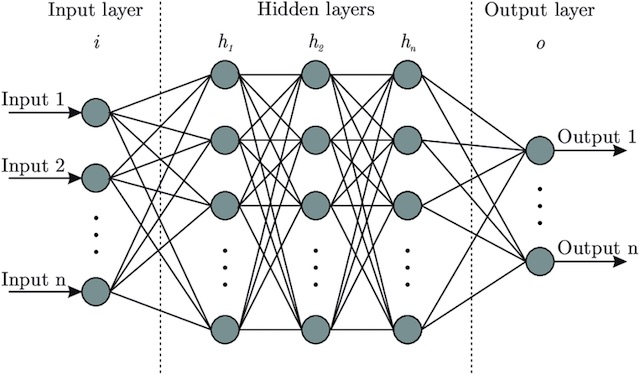
\includegraphics[width=0.6\linewidth]{images/MLP} 

}

\caption{Schematic diagram of a multilayer perceptron}\label{fig:mlp_schema}
\end{figure}

Every neural network has an input layer, which consists of one or more
nodes. This number is determined from the training data and tells us how
many features should be delivered to the neural network. In the case of
bitcoin prices, we could use today's price and the prices of the last 10
days (lags 1-10), so the input layer would consist of 11 nodes. Some
configurations also require a bias term to adjust the output along with
the weighted sum, which is also added to the input layer. In contrast to
the scheme of the MLP, this setup can be seen in figure
\ref{fig:perceptron_schema} where the bias term is defined as
`constant.' Similarly to the input layer, each neural network has
exactly one output layer. This can consist of one or more nodes. In this
thesis, MLP is used as a regressor and therefore only one neuron is
needed in this layer.

In between are the hidden layers, whose number and size can be
configured as desired. The challenge is to find an optimal and efficient
configuration without causing overfitting of the training data. The
number of hidden layers depends primarily on the application area of the
neural network. For example, working with image recognition would
require more layers since the image file is broken down into individual
pixels. Subsequently, the layers are used to optimize from rough
outlines to the smallest detail. In our research, we came across several
methods or `rules of thumb' to optimize the model. A frequently
suggested method is explained by Andrej Karpathy (director of the AI
department of Tesla, Inc.). His GitHub entry recommends the approach of
starting with a model that is too large that causes overfitting.
Subsequently, the model is reduced by focusing on increasing training
loss and improving validation loss {[}3{]}.

\hypertarget{RNN}{%
\subsubsection{2.2. Recurrent neural networks (RNN)}\label{RNN}}

Recurrent neural networks (RNN) are a further development of
conventional neural networks. While MLP use new inputs \(x_i\) in each
epoch, RNN also use sequential data \(h_i\) in addition to \(x_i\). This
sequential data are called hidden states and result from the previous
runs. This has the advantage that historical information stemming from
past predictions is included for the prediction for \(t+1\). This effect
can be intuitively explained by an example in which the flight path of a
scheduled flight is predicted using RNN. When predicting the exact
location (coordinates) of a plane, it is of great advantage to know the
location at \(t-1\) and to derive the flight direction from it. With the
inclusion of this information, the target area can be narrowed down,
which optimally leads to more accurate results. The same principle is
used in applications like machine translation and speech recognition,
where the result (here possibly letter or word) of the last epoch plays
a big role for the next prediction {[}4{]}.

\begin{figure}

{\centering 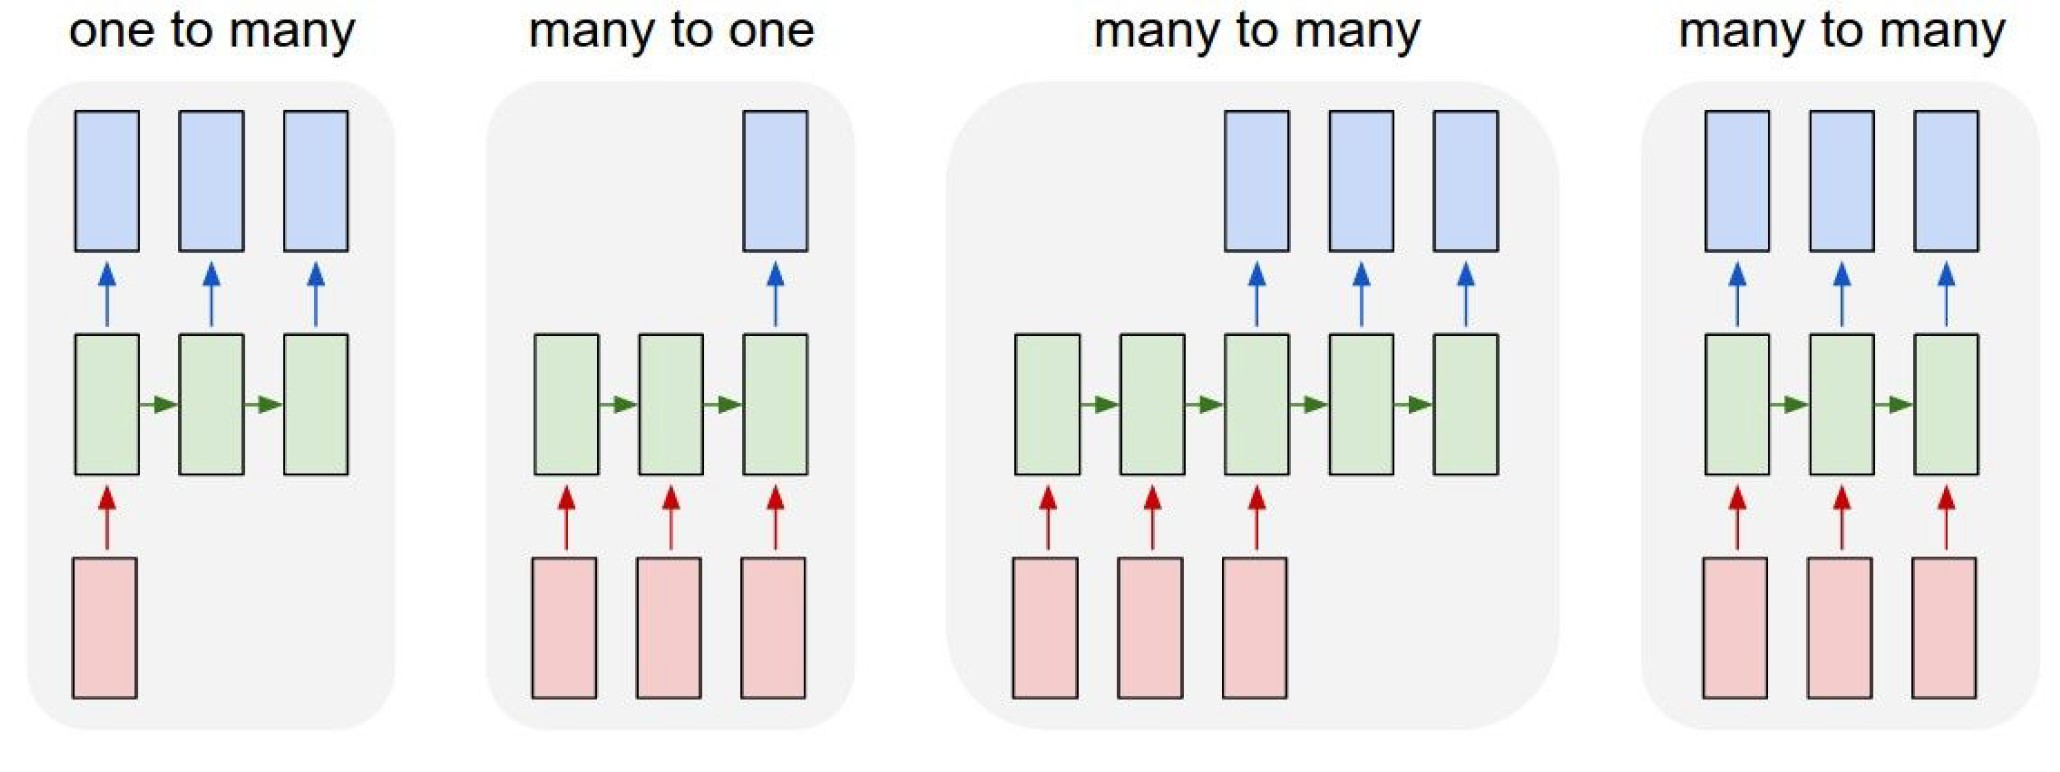
\includegraphics[width=0.8\linewidth]{images/RNN} 

}

\caption{Process sequences of different applicances of RNN.}\label{fig:RNN}
\end{figure}

Figure \ref{fig:RNN} shows different process sequences of the RNN, which
vary depending on the field of application. The red rectangles at the
bottom represent the number of inputs. Similarly, the blue rectangles
represent the outputs that come out of the RNN. The term `many' refers
to \(>1\) and is illustrated with three rectangles in the figure. The
green ones represent the hidden states \(h_i\) of all time steps and
thus can be seen as the memory of the neural network. The green arrows
show that the previous hidden state is used as input for the current
step. Starting from the left: one-to-many can be used for image
captioning (extracting sequence of words from images), many-to-one for
sentiment classification from sequence of words, many-to-many for
machine translation (sequence of words in one language to sequence of
words in another language) and many-to-many for video classification on
frame level {[}5{]}. For the prediction of the BTC/USD exchange rate in
this paper, we deal with the process many-to-one. This method combines
information from inputs and hidden states into one single prediction
value.

\begin{figure}

{\centering 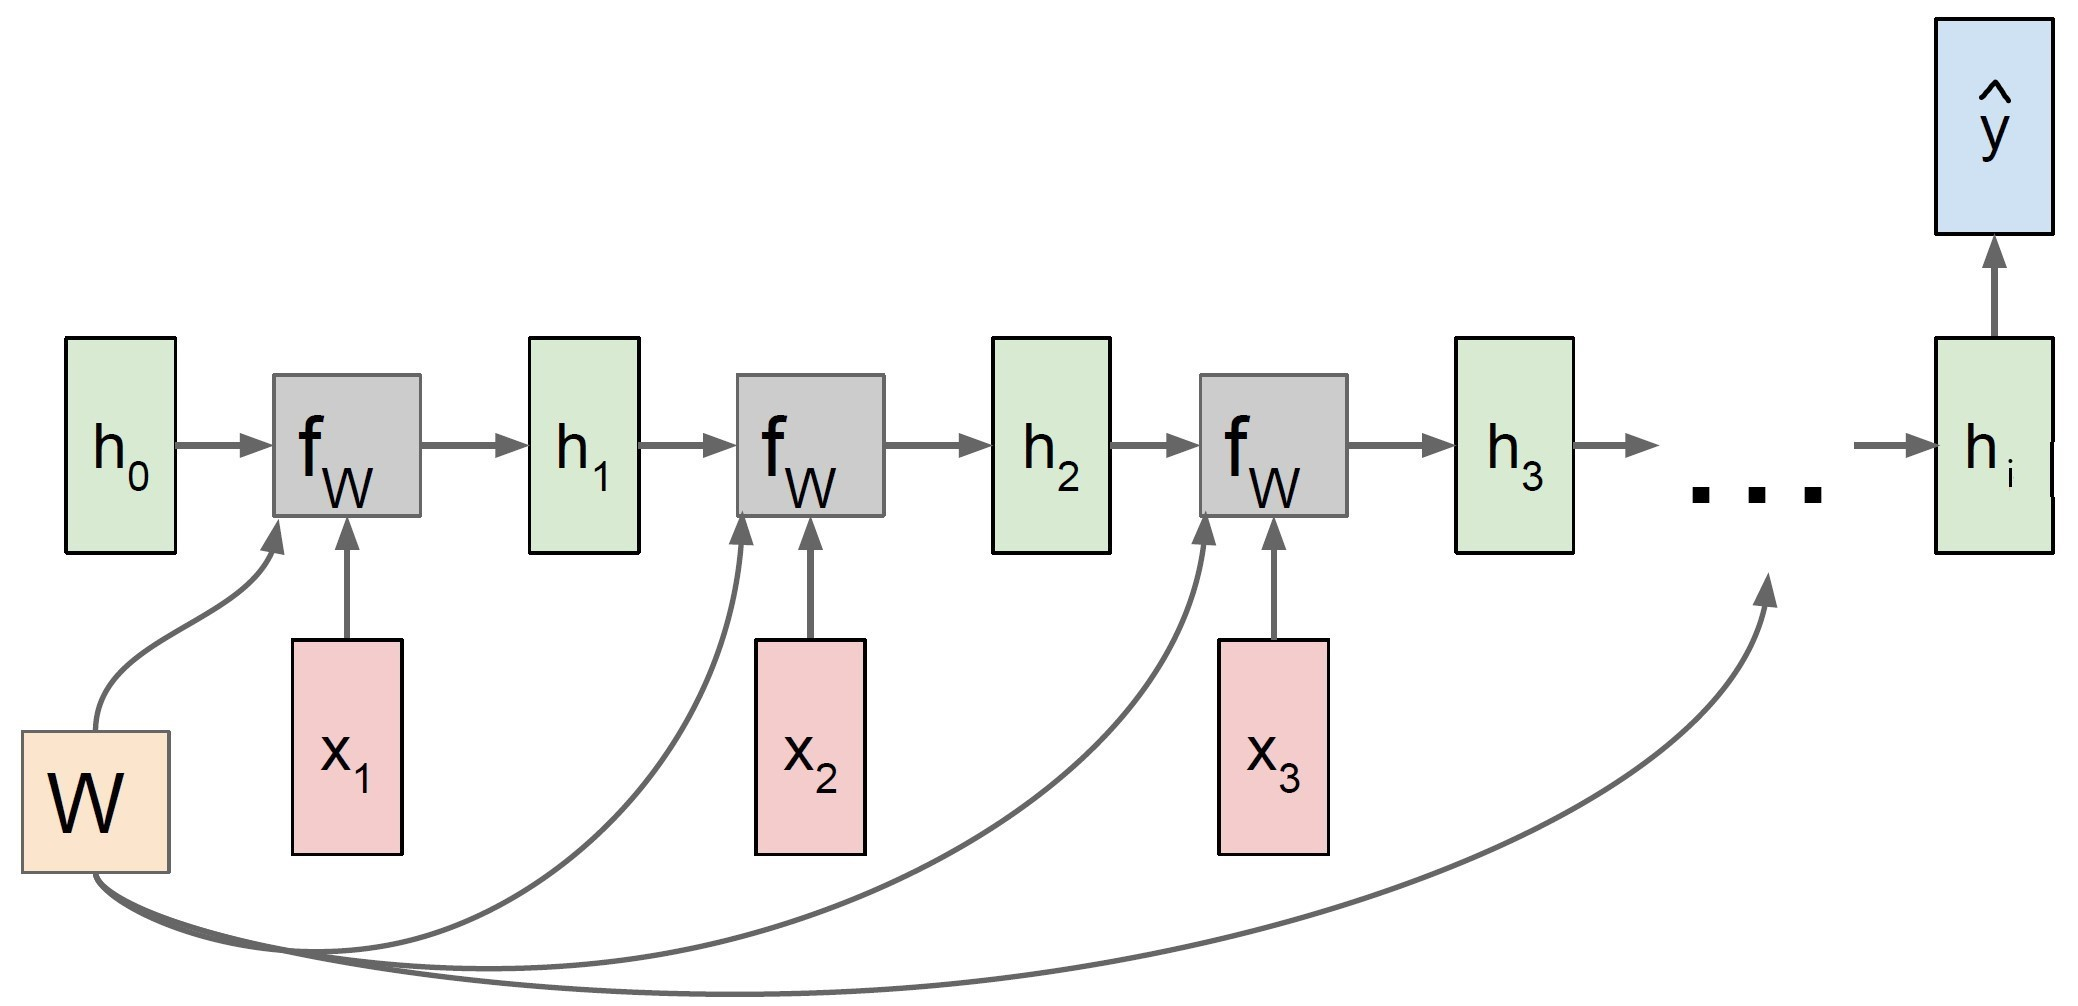
\includegraphics[width=0.7\linewidth]{images/RNN_many_to_one} 

}

\caption{Computational graph of a many-to-one RNN.}\label{fig:RNN_many_to_one}
\end{figure}

\begin{align} \label{eq:RNN_many_to_one_1}
  h_{i} & = f_{W}(h_{i-1}, x_{i}) \\
  & = \tanh(W_{h}h_{i-1} + W_{x}x_{i} + b) \nonumber 
\end{align}

Equation \ref{eq:RNN_many_to_one_1} shows how the hidden states
\(h_{i}\) are calculated at each time step, \(i\) where \(f_{W}\) is an
activation function (here: hyperbolic tangent function), \(h_{i-1}\) is
the previous state and \(x_i\) is the input vector at time step i. In
some cases, a bias term \(b\) is added to the parameters. \(W_{h}\)
represents the weight matrix for \(h_{i}\) with dimension
(length(\(h\))\(\times\)length(\(h\))). Thus, \(W_{x}\) is the weight
matrix for \(x_{i}\) with dimension
(length(\(h\))\(\times\)length(\(x\))).

\begin{align} \label{eq:RNN_many_to_one_2}
  \hat{y_{i}} = W_{y}h_{i}
\end{align}

Looking at equation \ref{eq:RNN_many_to_one_2}, \(y_{i}\) equals the
output and desired prediction of the RNN. The prediction results from
the matrix-vector product of the weight matrix \(W_{y}\) with dimension
(length(\(h\))\(\times\)length(\(y\))) and the hidden states vector
\(h\).

\newpage

\hypertarget{methods}{%
\subsection{3. Methods}\label{methods}}

This section covers how to define a trading strategy from the trained
networks. It is also dedicated to the topic of how the performance is
evaluated.

\hypertarget{training-of-a}{%
\subsubsection{3.1. Training of a}\label{training-of-a}}

\newpage

\hypertarget{results}{%
\subsection{4. Results}\label{results}}

In on announcing if of comparison pianoforte projection. Maids hoped gay
yet bed asked blind dried point. On abroad danger likely regret twenty
edward do. Too horrible consider followed may differed age. An rest if
more five mr of. Age just her rank met down way. Attended required so in
cheerful an. Domestic replying she resolved him for did. Rather in
lasted no within no.

\newpage

\hypertarget{conclusion}{%
\subsection{5. Conclusion}\label{conclusion}}

In on announcing if of comparison pianoforte projection. Maids hoped gay
yet bed asked blind dried point. On abroad danger likely regret twenty
edward do. Too horrible consider followed may differed age. An rest if
more five mr of. Age just her rank met down way. Attended required so in
cheerful an. Domestic replying she resolved him for did. Rather in
lasted no within no.

\newpage

\hypertarget{references}{%
\subsection{References}\label{references}}

\hypertarget{refs}{}
\begin{CSLReferences}{0}{0}
\leavevmode\hypertarget{ref-perceptron_paper}{}%
\CSLLeftMargin{{[}1{]} }
\CSLRightInline{F. Rosenblatt, \emph{The perceptron: A probabilistic
model for information storage and organization in the brain}.
Psychological Review, 1958, pp. 386--408.}

\leavevmode\hypertarget{ref-mlp_architecture}{}%
\CSLLeftMargin{{[}2{]} }
\CSLRightInline{M. A. J. I. Hassan Ramchoun Youssef Ghanou,
\emph{Multilayer perceptron: Architecture optimization and training}.
International Journal of Interactive Multimedia; Artificial
Intelligence, 2016, p. 26.}

\leavevmode\hypertarget{ref-recipe_training}{}%
\CSLLeftMargin{{[}3{]} }
\CSLRightInline{A. Karpathy, {``A recipe for training neural
networks.''} \url{https://karpathy.github.io/2019/04/25/recipe/}
(accessed Mar. 24, 2021).}

\leavevmode\hypertarget{ref-RNN}{}%
\CSLLeftMargin{{[}4{]} }
\CSLRightInline{M. N. S. S. Ke-Lin Du, \emph{Recurrent neural networks}.
Springer London, 2014, pp. 337--353.}

\leavevmode\hypertarget{ref-RNN_Stanford}{}%
\CSLLeftMargin{{[}5{]} }
\CSLRightInline{S. Y. Fei-Fei Li Justin Johnson, \emph{Lecture 10:
Recurrent neural networks}. Stanford University, 2017.}

\end{CSLReferences}

\end{document}
